\documentclass{standalone}

\usepackage{tikz}
\usetikzlibrary{patterns,arrows,calc,decorations.pathmorphing,backgrounds, positioning,fit,petri,decorations.fractals,trees, matrix}
\usetikzlibrary{shapes}
\usepackage{amsmath, amsfonts}

\begin{document}
	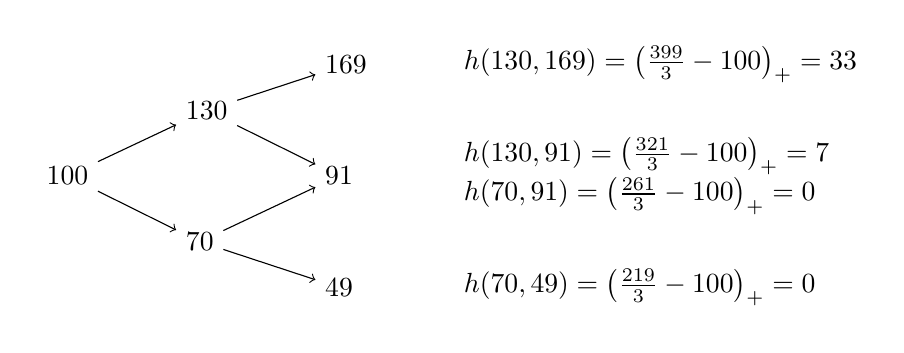
\begin{tikzpicture}
		\matrix (tree) [matrix of nodes,column sep=1cm, nodes={anchor=west}]
		{
			      &              & $169$ & $h(130,169) = \left( \frac{399}{3} - 100 \right)_+ = 33$ \\
			      & $130$  &                  \\
			$100$ &              & $91$ & \parbox{5cm}{ %
				$h(130,91) = \left( \frac{321}{3} - 100 \right)_+ = 7$ \\
				$h(70,91) = \left( \frac{261}{3} - 100 \right)_+ = 0$%
			} \\
			      & $70$  &                  \\
				  &              & $49$    & $h(70,49) = \left( \frac{219}{3} - 100 \right)_+ = 0$ \\
		};
		\draw[->] (tree-3-1)--(tree-2-2);
		\draw[->] (tree-3-1)--(tree-4-2);
		%%
		\draw[->] (tree-2-2)--(tree-1-3);
		\draw[->] (tree-2-2)--(tree-3-3);
		\draw[->] (tree-4-2)--(tree-3-3);
		\draw[->] (tree-4-2)--(tree-5-3);
		
	\end{tikzpicture}

\end{document}